\chapter{Introduction au Réseaux de Neurones Artificiels}
\chapterintrobox{Les réseaux neuronaux artificiels sont des systèmes de computation capables de trouver des fonctions complexes qui relient une entrée à une sortie. ces systèmes peuvent être utilisés pour une variété de tâches comme la régression et la classification. Ils peuvent être utilisés dans le domaine de la maintenance prédictive et des pronostics pour estimer l'état de santé de l'équipement et prévoir avec une certaine incertitude sa durée de vie utile restante. Ce chapitre traite les réseaux de neurones, leur topologie, leur entraînement et leur formulation mathématique.}


\section{La structure de réseaux de neurones artificiels}
Les réseaux de neurones artificiels sont des systèmes de computation utilisés pour trouver la correspondance entre une entrée et une sortie, ils sont constitués de plusieurs couches (couche d'entrée, couche de sortie et un nombre arbitraire de couches cachées entre l'entrée et la sortie) et chaque couche contient un certain nombre de neurones où chaque neurone de chaque couche est connecté à tous les neurones de la couche précédente et de la couche suivante (à l'exception des couches d'entrée et de sortie qui sont connectées uniquement aux couches suivante et précédente respectivement).
chaque neurone de chaque couche reçoit une entrée des neurones de la couche précédente (sous la forme d'un vecteur), multiplie le vecteur par quelques poids et somme le résultat puis applique une fonction d'activation linéaire. Chaque neurone se retrouve avec une seule valeur numérique appelée activation, qui sera transmise aux neurones de la couche suivante.

Figure \ref{fig:neural-network-structure} montre un réseau de neurones avec la structure suivante :

\begin{itemize}
    \item Une couche d'entrée avec 3 entrée
    \item Une seule couche cachée avec 4 neurones
    \item Une couche de sortie avec 1 neurone 
\end{itemize}

\begin{figure}[h]
    \centering
	

	
		
		
\begin{tikzpicture}[neuron/.style={circle,draw, thick,align=center, minimum size=2em,inner sep=1pt}, input/.style={->}]

\node[text width=2cm, align=center] at (0,.5*\nodedist) {\small Input Layer};

\node[text width=2cm, align=center] at (\layerdist,.5*\nodedist) {\small Hidden Layer};

\node[text width=2cm, align=center] at (2*\layerdist,.5*\nodedist) {\small Output Layer};

\foreach \y in {1,...,3} \node[] (in\y) at (-\layerdist*.5,-\y*\nodedist) {$x_\y^{(i)}$};  

\foreach \y in {1,...,3} \node[neuron]  (I\y) at (0,-\y*\nodedist) {$a_\y^{[1]}$};  

\foreach \in in {1,...,3} \draw[->, >=angle 60] (in\in) --  (I\in);

\foreach \y in {1,...,4} \node[neuron]  (H\y) at ($(\layerdist,-\y*\nodedist) +(0, .5*\nodedist)$) {$a_\y^{[2]}$};

\foreach \y in {1,...,1} \node[neuron] (O\y) at ($(I2) + (2*\layerdist, 0)$) {$a_\y^{[3]}$};

\node at ($(I2) + (2.5*\layerdist, 0)$) (y) {$\hat{y}^{(i)}$};


\foreach \dest in {1,...,4} \foreach \source in {1,...,3} \draw[->, >=angle 60] (I\source) -- (H\dest);

\foreach \dest in {1,...,1} \foreach \source in {1,...,4} \draw[->, >=angle 60] (H\source) -- (O\dest);

\draw[->, >=angle 60] (O1) -- (y);

%\draw[->,  thick, >=angle 60] (.5*\layerdist,-4.5*\nodedist) -- node[above] {Direction of forward propagation} (1.5*\layerdist,-4.5*\nodedist);
%\draw[->,  thick, >=angle 60]  (1.5*\layerdist,-4.8*\nodedist)-- node[below] {Direction of backpropagation} (.5*\layerdist,-4.8*\nodedist);
%\node [anchor=west] (note) at (-1.3*\layerdist,-4*\nodedist) {\footnotesize Single neuron};
%\draw [->,  thick, >=angle 60] (note) to[out=0, in=-120] (I3.south);
\end{tikzpicture}
		
		

    \caption{Structure d'un réseau de neurones}
    \label{fig:neural-network-structure}
\end{figure}

\section{Feedforward: de l'entrée vers la sortie}
\label{section:feedforward-neural-network}
L'architecture de la figure \ref{fig:neural-network-structure} est appelée Feedforward Neural Network, c'est une architecture acyclique où l'information circule de la première à la dernière couche sans aucune boucle interne, contrairement aux autres architectures comme les réseaux de neurones récurrents. La première couche est la couche d'entrée, elle n'effectue aucune opération et se limite à recevoir l'entrée. L'entrée est un vecteur de nombres représente les différentes variables. Le vecteur est multiplié par une matrice de poids qui le transforme et l'envoie à la couche suivante (ou à la première couche cachée). Une fonction d'activation est appliquée aux valeurs résultant de la multiplication des valeurs de la couche précédente avec la matrice des poids, le résultat devient les valeurs de la couche suivante, ou activations (la valeur de chaque neurone est appelée activaiton).

Une formule générale pour passer de la couche $l-1$ à la couche $l$ est donnée par l'équation \ref{equation:forward-step}:

\begin{equation}
    a^{[l]} = g^{[l]}(W^{[l]}a^{[l-1]}+b^{[l]})
    \label{equation:forward-step}
\end{equation}

Où $g^{[l]}$ est la fonction d'activation de la couche $l$, $W^{[l]}$ est la matrice des poids qui transforme les valeurs (activations) de la couche $l-1$ à la couche $l$ et $a^{[l]}$ représente les activations de la couche $l$. $b$ est la valeur du biais (ou valeur d'interception), elle est ajoutée à la multiplication entre les activations et la matrice des poids, c'est un paramètre qui peut être appris comme les poids. L'opération se répète pour chaque couche jusqu'à la couche de sortie.
La première couche peut être considérée comme la couche 0 et les entrées peuvent être désignées par le vecteur $a^{[0]}$.

\section{Fonction d'activation}
Les fonctions d'activation sont appliquées au résultat de la multiplication des entrées de la couche précédente avec les poids correspondants, pour déterminer la valeur de chaque neurone. Il existe différents types de ces fonctions.

L'utilisation de la fonction d'activation non linéaire est très importante pour les réseaux de neurones, ils permettent d'apprendre la correspondance non linéaire complexe de l'entrée à la sortie. Si le réseau n'utilise pas l'activation non linéaire (par exemple, l'activation linéaire ou la fonction d'identité), alors le réseau entier (quelle que soit sa profondeur) est équivalent à un réseau avec une seule couche cachée.

Il existe une variété de fonctions d'activation qui peuvent être utilisées pour les couches cachées et de sortie. La figure \ref{fig:activation-function} montre quelques examples:

\begin{figure}[h]
    \centering
	\begin{subfigure}[b]{0.24\linewidth}


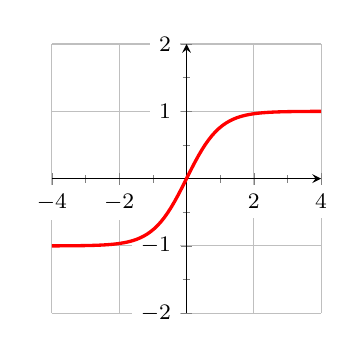
\begin{tikzpicture}
	\begin{axis}[ 
%title=$\tanh(x)$,
xmin=-4, xmax=4,ymin=-2, 
ymax=2, grid=major,
height=5cm, width=5cm,
axis line style={latex-latex},
axis lines=middle,
ticklabel style={font=\footnotesize,fill=white},
minor tick num=1,
scaled ticks=false] 
\addplot[samples=100,red,very thick] {tanh(x))};
%\addlegendentry{$\tanh(x)$}
\end{axis}
\end{tikzpicture} 
\subcaption{tanh}
\end{subfigure}
\hfill
\begin{subfigure}[b]{0.24\linewidth}



	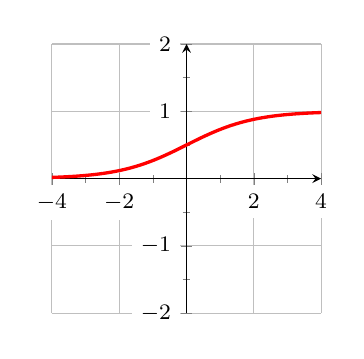
\begin{tikzpicture}
	\begin{axis}[ 
	%title=$\tanh(x)$,
	xmin=-4, xmax=4,ymin=-2, 
	ymax=2, grid=major,
	height=5cm, width=5cm,
	axis line style={latex-latex},
	axis lines=middle,
	ticklabel style={font=\footnotesize,fill=white},
	minor tick num=1,
	scaled ticks=false] 
	\addplot[samples=100,red,very thick] {1/(1+exp(-x))};
	%\addlegendentry{$\tanh(x)$}
	\end{axis}
	\end{tikzpicture}
	
	
	
\subcaption{sigmoid}
\end{subfigure}
\hfill
	\begin{subfigure}[b]{0.24\linewidth}
		
		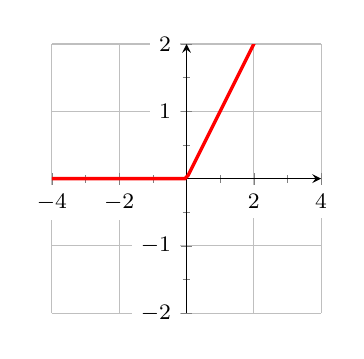
\begin{tikzpicture}
		\begin{axis}[ 
		%title=$\tanh(x)$,
		xmin=-4, xmax=4, ymin=-2, ymax=2, grid=major,
		height=5cm, width=5cm,
		axis line style={latex-latex},
		axis lines=middle,
		ticklabel style={font=\footnotesize,fill=white},
		minor tick num=1,
		scaled ticks=false] 
		\addplot[samples=100,red,very thick] {max(0,x)};
		%\addlegendentry{$\tanh(x)$}
		\end{axis}
		
		\end{tikzpicture}

\subcaption{ReLU}
	\end{subfigure}
\hfill
		\begin{subfigure}[b]{0.24\linewidth}
			
		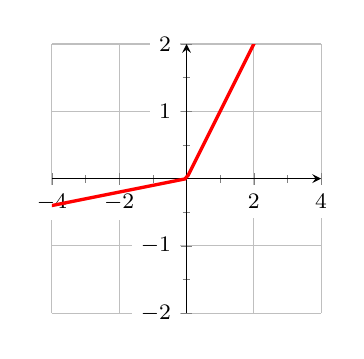
\begin{tikzpicture}
		\begin{axis}[ 
		%title=$\tanh(x)$,
		xmin=-4, xmax=4,ymin=-2, 
		ymax=2, grid=major,
		height=5cm, width=5cm,
		axis line style={latex-latex},
		axis lines=middle,
		ticklabel style={font=\footnotesize,fill=white},
		, xticklabel style={anchor=north},
		minor tick num=1,
		scaled ticks=false] 
		\addplot[samples=100,red,very thick] {max(0,x)+min(0,0.1*x)};
		%\addlegendentry{$\tanh(x)$}
		\end{axis}
		
		\end{tikzpicture}
		\subcaption{Leaky ReLU}
		\end{subfigure}
    \caption{Différentes fonctions d'activation}
    \label{fig:activation-function}
\end{figure}

Tablea \ref{table:activation-functions} montre les définition mathematiques de quelques fonctions d'activation:

\begin{table}[h]
    \centering
    \begin{tabular}{c|c}
        \hline
        Fonction d'activation & Défnition mathématique \\
        \hline
        Identity (pas d'activation) & Id(x) = x \\
        Sigmoid & $\sigma(x)= \frac{1}{1+e^{-x}}$ \\
        tanh & $tanh(x)=\frac{(e^x-e^{-x})}{(e^x+e^{-x})}$\\
        Rectified Linear Unit (ReLU) & $ReLU(x)=max(0,x)$\\
        Leaky ReLU & $LeakyReLU(x)=max(0.1 x,x)$\\
    \hline
        
    \end{tabular}
    \caption{Définitions mathématiques de quelques fonctions d'activation}
    \label{table:activation-functions}
\end{table}

\section{Entraînement du réseau}
Le processus de formation d'un réseau de neurones consiste à déterminer les poids (coefficients) qui relient les neurones de chaque couche aux neurones de la couche suivante. Ce processus peut être formulé en termes plus mathématiques comme un problème d'optimisation : optimisation des coefficients du réseau pour trouver leurs valeurs qui minimisent une fonction de coût.

L'entraînement du réseau de neurones utilise des données d'entraînement (training data) qui fournissent des entrées et leurs sorties correspondantes.

\subsection{Fonction de coût}
La fonction de coût est la fonction utilisée pour calculer la différence entre la sortie du réseau de neurones et la sortie réelle attendue, elle quantifie la performance du réseau. Le but du processus d'entraînement est de minimiser cette fonction en utilisant Gradient Descent (voir la section suivante) pour trouver le meilleur ensemble de poids qui donne la différence la plus basse entre les données d'entraînement et la prédiction du réseau.

Il existe de nombreux types de fonctions de coût, chaque type correspondant à différentes tâches des réseaux de neurones (par exemple, régression, classification binaire, ...). La fonction de coût généralement utilisée pour les problèmes de régression est une fonction d'erreur quadratique moyenne (Equation \ref{equation:mse}) qui calcule la somme des distances entre les prédictions du modèle $\hat{y}_i$ et la sortie réelle ($y_i$), $N$ le nombre de points de données disponibles pour l'entraînement :

\begin{equation}
    MSE=\frac{1}{N}\sum_{i=1}^N(y_i-\hat{y}_i)
    \label{equation:mse}
\end{equation}

L'autre principale tâche des réseaux de neurones et des autres types de modèles est la classification. Il existe deux principaux types de classification : la classification binaire, ou classification de deux classes et la classification multiclasse ou classification de plusieurs classes. La première utilise la fonction de perte d'entropie croisée binaire (Equation \ref{equation:logloss}) et la seconde utilise l'entropie croisée catégorielle.

\begin{equation}
    BCE = \sum_{i=1}^{N}\hat{y}_i log(y_i)+(1-\hat{y}_i)log(1-\hat{y}_i)
    \label{equation:logloss}
\end{equation}

Le choix de la fonction d'activation pour la dernière couche du réseau est directement lié à la fonction de coût utilisée. Pour les tâches de régression, la fonction d'activation linéaire est utilisée. Pour la classification binaire, c'est la fonction sigmoïde et pour la classification multiclasse, c'est la fonction softmax.

\subsection{Gradient Descent}
Gradient Descent est un algorithme d'optimisation itératif utilisé pour optimiser une fonction différentiable. Gradient Descent fonctionne en calculant les gradients de la fonction objectif puis en prenant des mesures itératives dans le sens du négatif des gradients.

\subsection{Convex and non-convex functions}
Gradient descent in neural networks is used to optimize (minimize) the cost function by finding the best set of weights and biases that give the lowest cost possible. Objective functions can be categorized into two types: convex and non-convex functions.
A convex function is said to be convex if it has the property that every chord lies on or above the function. Any value of $x$ in the interval from $x=a$ to $x=b$ can be written in the form $\lambda a+(1-\lambda)b$ where $0\leq\lambda\leq 1$. The corresponding point on the chord is given by $\lambda f(a)+(1-\lambda)f(b)$, and the corresponding value of the function is $f(\lambda a+(1-\lambda)b)$ (Figure \ref{fig:convexity}). Convexity then implies:
\begin{equation}
    f(\lambda a+(1-\lambda)b)\leq \lambda f(a)+(1-\lambda)f(b)
    \label{equation:convexity}
\end{equation}

This is equivalent to the requirement that the second derivative of the function be everywhere positive \cite{Bishop2006}. This condition of convexity can be extended to spaces with arbitrariliy large number of dimensions.

\begin{figure}[h]
    \centering
    \includegraphics{figures/convex_function.pdf}
    \caption{Condition of convexity}
    \label{fig:convexity}
\end{figure}

A non-convex function is a funciton that doesn't satisfy the convexity condition. Figure \ref{fig:convex-nonconvex-functions} shows an example of a convex (left) and a non-convex function (right) where the function parameters are in two-dimensional space.

\begin{figure}[h]
    \centering
    \includegraphics{figures/gradient_descent.pdf}
    \caption{Example of convex and non-convex functions}
    \label{fig:convex-nonconvex-functions}
\end{figure}


\subsection{Global and local minima}
Global minimum refers to the lowest possible value in a set (or of a function). Finding the global minimum refers to finding the set of parameters that correspond to this minimum value. When the function is convex, finding the global maximum is possible and easy, algorithms like gradient descent always converge to the global minimum in convex optimization. Examples of convex cost functions is linear regression cost function. For more complex models such as neural networks, cost function is highly non-convex with many local minima.

Figure \ref{fig:global_local_minima} shows an example of a non-convex function with a global and local minima. The problem with non-convex optimization is that the optimization algorithm can converge to the local minimum instead of the global one. The algorithm convergence is related to the random initialization of network weights.

\begin{figure}[h]
    \centering
    \includegraphics{figures/global_local_minima.pdf}
    \caption{Non-convex function with global and local minima}
    \label{fig:global_local_minima}
\end{figure}

\subsection{Saddle points}
A saddle point or minimax point is a point on the surface of the graph of a function where the slopes (derivatives) in orthogonal directions are all zero (a critical point), but which is not a local extremum of the function (Figure \ref{fig:saddle-point}).

\begin{figure}[h]
    \centering
    \includegraphics{figures/saddle_point.pdf}
    \caption{Saddle point}
    \label{fig:saddle-point}
\end{figure}

\subsection{Optimization of multilayer networks}
In  \cite{Choromanska2014} the authors showed that getting stuck in poor local minima is a major problem for smaller networks but becomes gradually of less importance as the network size increases. This is because critical points of large networks exhibit the layered structure where high-quality low-index critical points lie close to the global minimum.

The following hypotheses were also verified empirically in the mentioned paper regarding learning with large-size networks:
\begin{itemize}
    \item For large-size networks, most local minima are equivalent and yield similar performance on a test set.
    \item The probability of finding a “bad” (high value) local minimum is non-zero for small-size networks and decreases quickly with network size.
    \item Struggling to find the global minimum on the training set (as opposed to one of the many good local ones) is not useful in practice and may lead to overfitting.
\end{itemize}

\subsection{Backpropagation}
Backpropagation est l'algorithme utilisé pour calculer les gradients de la fonction de coût (la fonction objectif) d'un réseau de neurones. Comme un réseau de neurones peut être interprété comme une fonction composite, Backpropagation utilise le théorème de dérivation des fonctions composées
pour trouver les gradients par rapport aux poids du réseau.

L'utilisation de Backpropagation pour l'entraînement de réseaux de neurones a été popularisée par David E. Rumelhart, Geoffrey E. Hintont et Ronald J. Williams \cite{Rumelhart1986}, ils l'ont décrit comme une procédure qui ajuste de manière répétée les poids des connexions du réseau de manière à minimiser une mesure de la différence entre le vecteur de sortie réel du réseau et le vecteur de sortie souhaité. À la suite des ajustements de poids, des unités internes "cachées" qui ne font pas partie de l'entrée ou de la sortie en viennent à représenter des caractéristiques importantes du domaine de la tâche, et les régularités de la tâche sont saisies par les interactions de ces unités.

Figure \ref{fig:forward-backward-pass} représente le Forward Pass et le Backward Pass, le Forward Pass calcule la sortie de réseau, le Backward pass calcule les gradients de la fonction de coût qui mesure la difference entre cette sortie et la sortie réelle souhaitée:

\begin{figure}[h]
    \centering
	\documentclass[12pt]{article}
\usepackage{tikz}
\usetikzlibrary{arrows,positioning}
\begin{document}
	

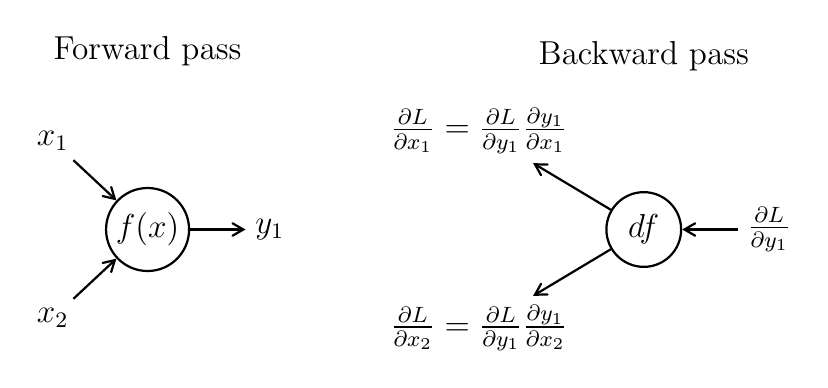
\begin{tikzpicture}[arrow/.style={thick, >=angle 60}]
	\node[draw, circle,thick,minimum width=3em, inner sep=0] (fp) {\large $f(x)$};
	\node[above left = 2em of fp] (x1) {\large $x_1$};
	\node[below left = 2em of fp] (x2) {\large $x_2$};
	\node[right = 2em of fp] (y1) {\large $y_1$};
	
	\node[above = 4em of fp] {\large Forward pass};
	
	\draw[->,arrow] (x1) -- (fp);
	\draw[->,arrow] (x2) -- (fp);
	\draw[->,arrow] (fp) -- (y1);

\node[draw, circle,thick,minimum width=2.7em, inner sep=0, right = 15 em of fp] (bp) {\large $df$};
\node[above left = 2em of bp] (bx1) {\large $\frac{\partial L}{\partial x_1}=\frac{\partial L}{\partial y_1}\frac{\partial y_1}{\partial x_1}$};

\node[below left = 2em of bp] (bx2) {\large $\frac{\partial L}{\partial x_2}=\frac{\partial L}{\partial y_1}\frac{\partial y_1}{\partial x_2}$};

\node[right = 2em of bp] (by1) {\large $\frac{\partial L}{\partial y_1}$};

\node[above = 4em of bp] {\large Backward pass};

\draw[<-,arrow] (bx1) -- (bp);
\draw[<-,arrow] (bx2) -- (bp);
\draw[<-,arrow] (bp) -- (by1);
\end{tikzpicture}
	
\end{document}
    \caption{Forward (gauche) et Backward (droite) passes}
    \label{fig:forward-backward-pass}
\end{figure}


\section{Réseaux de neurones récurrents}
Les réseaux de neurones récurrents (\acrshort{rnn}) sont une architecture spéciale qui convient mieux à la modélisation de données séquentielles. Les \acrshort{rnn} traitent une séquence d'entrée un élément à la fois, en maintenant dans leurs unités cachées un "vecteur d'état" qui contient implicitement des informations sur l'historique de tous les éléments passés de la séquence \cite{LeCun2015}. Figure \ref{fig:rnn} montre une architecture \acrshort{rnn}. À gauche, on voit la version dépliée avec une boucle cyclique dans la couche cachée et à droite la version déroulée. $x_1$, $x_2$, …$x_t$ représentent le vecteur d'entrée (séquence), $y_1$, $y_2$, …$y_t$ est le vecteur de sortie (peut être une séquence de longueur égale à l'entrée, de longueur différente ou un seul élément). $h_1$, $h_2$, …$h_t$ sont les neurones de la couche cachée, chaque neurone passe un vecteur de son état caché au neurone suivant.

\begin{figure}[H]
    \centering
    	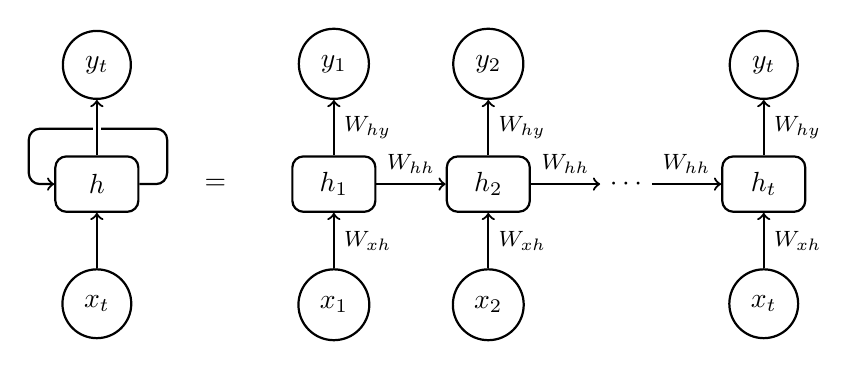
\begin{tikzpicture}[layer/.style={rectangle,draw, thick,align=center, minimum width=3em, minimum height=2em,inner sep=5pt,rounded corners=4},neuron/.style={circle,draw, thick,align=center,inner sep=5pt,rounded corners=4}, links/.style={->, thick}]
	
	\node[layer] (h-rolled) {$h$};
	\node[neuron, below = 2em of h-rolled] (input-rolled) {$x_t$};
	\node[neuron, above = 2em of h-rolled] (output-rolled) {$y_t$};
		\draw[links, rounded corners] (h-rolled.east) -| ++(1em,2em) -- ++(-5em,.0em) |- (h-rolled.west);
	\draw[links] (input-rolled) -- (h-rolled);
	\draw[line width=3pt,white] (h-rolled) -- (output-rolled);
	\draw[links] (h-rolled) -- (output-rolled);
	

	\node[right = 2em of h-rolled] (equals) {$=$};
	

	\node[layer, right = 2em of equals] (h-unrolled1) {$h_1$};
		\node[neuron, below = 2em of h-unrolled1] (input-unrolled1) {$x_1$};
	\node[neuron, above = 2em of h-unrolled1] (output-unrolled1) {$y_1$};
	\draw[links] (h-unrolled1) -- node[right] {\footnotesize $W_{hy}$} (output-unrolled1);
	\draw[links] (input-unrolled1) -- node[right] {\footnotesize $W_{xh}$} (h-unrolled1);
	
	
	
	\node[layer, right = 2.5em of h-unrolled1] (h-unrolled2) {$h_2$};
	\node[neuron, below = 2em of h-unrolled2] (input-unrolled2) {$x_2$};
	\node[neuron, above = 2em of h-unrolled2] (output-unrolled2) {$y_2$};
	
	\draw[links] (h-unrolled2) -- node[right] {\footnotesize $W_{hy}$} (output-unrolled2);
	\draw[links] (input-unrolled2) -- node[right] {\footnotesize $W_{xh}$} (h-unrolled2);
	
	\draw[links] (h-unrolled1) -- node[above] {\footnotesize $W_{hh}$} (h-unrolled2) ;
	
	\node[right = 2.5em of h-unrolled2] (dots) {$\cdots$}; 
	
	\draw[links] (h-unrolled2) -- node[above] {\footnotesize $W_{hh}$}(dots);
	
	\node[layer, right = 2.5em of dots] (h-unrolled3) {$h_t$};
	\node[neuron, below = 2em of h-unrolled3] (input-unrolled3) {$x_t$};
	\node[neuron, above = 2em of h-unrolled3] (output-unrolled3) {$y_t$};
	
	\draw[links] (h-unrolled3) -- node[right] {\footnotesize $W_{hy}$} (output-unrolled3);
	\draw[links] (input-unrolled3) -- node[right] {\footnotesize $W_{xh}$} (h-unrolled3);
	
	\draw[links] (dots) -- node[above] {\footnotesize $W_{hh}$}(h-unrolled3);
	
	\end{tikzpicture}

    \caption{Recurrent neural networks architecture}
    \label{fig:rnn}
\end{figure}

\subsection{Long Short-Term Memory}
\label{section:lstm}
Simple \acrshort{rnn}s have problems with learning long-term dependencies (i.e. making predictions based on predictions made many steps previously in the past) and vanishing gradients. \acrlong{lstm} (\acrshort{lstm}) was first introduced by Jürgen Schmidhuber and Sepp Hochreiter \cite{Hochreiter1997}. \acrshort{lstm} overcomes problems with basic \acrshort{rnn} by using what is called a cell state which enables \acrshort{lstm} networks to learn long-term dependencies. \acrshort{lstm} cells also possess three types of gates which together control the flow of information inside the cell:
\begin{itemize}
    \item \textbf{Forget gate}: Controls which information are kept or discarded at time $t$
    \item \textbf{Input gate}: Controls which information to store in the cell state at time $t$
    \item \textbf{Output gate}: Controls the final output of the cell at time $t$
\end{itemize}

Input, forget and output gates values are calculated using Equations \ref{equation:lstm_input_gate}, \ref{equation:lstm_forget_gate} and \ref{equation:lstm_output_gate} respectively:

\begin{align}
i_t &= \sigma(W_{xi}x_t + W_{hi}h_{t-1}+W_{ci}c_{t-1}+b_i) \label{equation:lstm_input_gate}\\
f_t &= \sigma(W_{xf}x_t + W_{hf}h_{t-1}+W_{cf}c_{t-1}+b_f) \label{equation:lstm_forget_gate}\\
o_t &= \sigma(W_{xo}x_t + W_{ho}h_{t-1}+W_{co}c_t+b_o) \label{equation:lstm_output_gate}\\
\end{align}

Input, forget and output gates are calculated at time $t$ using sets of weights and biases ($W_{xi}$, $W_{hi}$, $W_{ci}$, $b_i$), ($W_{xf}$, $W_{hf}$, $W_{cf}$, $b_f$) and ($W_{xo}$, $W_{ho}$, $W_{co}$, $b_o$) that controls how each of $x_t$, $h_{t-1}$ and $c_{t-1}$ affects the value of the gate respectively. A sigmoid function is used to convert the values to the range of 0 to 1. 

At each time step $t$, a candidate cell state $\tilde{c}_t$ is calculated using weights and a bias term ($W_{xc}$, $W_{hc}$, $b_c$) that maps the values of input $x_t$ and previous hidden state $h_{t-1}$ to the candidate cell state (Equation \ref{equation:lstm_candidate_cell_state}). As the name indicates, $\tilde{c}_t$ serves as a candidate to replace current cell state $c_t$ at time $t$. Cell state at time $t$ is obtained by using the forget gate to control which information are kept from the previous cell state and input gate to control which information are kept from the candidate cell state according to Equation \ref{equation:lstm_cell_state}. Final cell output is calculated using current cell state $c_t$ and output gate according to Equation \ref{equation:lstm_hidden_state}.

\begin{align}
    \tilde{c}_t &= tanh(W_{xc}x_t+W_{hc}h_{t-1}+b_c) \label{equation:lstm_candidate_cell_state} \\
    c_t &= f_tc_{t-1}+i_t\tilde{c}_t \label{equation:lstm_cell_state}\\
    h_t &= o_ttanh(c_t) \label{equation:lstm_hidden_state}
\end{align}

Gates control the flow of information inside the \acrshort{lstm} cell, their values range from 0 to 1 (sigmoid function) and control which information to keep and which to discard when updating the cell state (forget and input gates) and when calculating the \acrshort{lstm} cell output (output gate).

Figure \ref{fig:lstm} illustrates the different operations happening in a signle \acrshort{lstm} cell:

\begin{figure}[h]
    \centering
    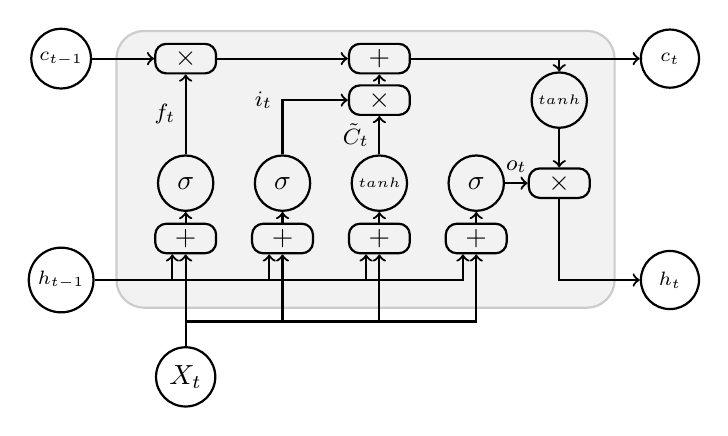
\begin{tikzpicture}

		\tikzstyle{operation} = [rectangle, thick,draw,align=center, minimum width=2.2em, minimum height=.5em,inner sep=2pt,rounded corners=4 ]
		
		\tikzstyle{links} = [->, thick]
		
		\tikzstyle{values} = [circle, draw, thick, inner sep = 2,minimum size=2.1em]
		
		\tikzstyle{functions} = [draw, circle, thick, inner sep=1, minimum size=20]
		
		\draw[rounded corners=10,black!20!white, thick, fill=black!5!white ] (0,0) rectangle (18em,-10em);
		
		\node[operation] at (2.5em, -7.5em) (addition1) {$+$};
		\node[operation] at (6em, -7.5em) (addition2) {$+$};
		\node[operation] at (9.5em, -7.5em) (addition3) {$+$};
		\node[operation] at (13em, -7.5em) (addition4) {$+$};
		
		
		\node[functions] at (2.5em, -5.5em) (sigma1) {$\sigma$};
		\node[functions] at (6em, -5.5em) (sigma2) {$\sigma$};
		\node[functions] at (9.5em, -5.5em) (tanh1) {\tiny $tanh$};
		\node[functions] at (13em, -5.5em) (sigma3) {$\sigma$};
		
		
		\node[operation] at (9.5em, -2.5em) (times1) {$\times$};
		\node[operation] at (9.5em, -1em) (addition5) {$+$};
		
		\node[operation] at (16em, -5.5em) (times2) {$\times$};
		\node[functions] at (16em, -2.5em) (tanh2) {\tiny $tanh$};
		
		\node[operation] at (2.5em, -1em) (times3) {$\times$}; 
		
		\node[circle, draw, thick, inner sep = 2.5] at (2.5em, -12.5em) (input) {$X_t$};
		
		
		
	%	\node[circle, draw, thick, inner sep = 2.5, left = 2.5em of times3] (previouscellstate) {\scriptsize $c_{t-1}$} ;
		
		\node[values] at (-2em,-1em) (previouscellstate) {\scriptsize $c_{t-1}$} ;
		
		\node[values] at (-2em,-9em) (previoushiddenstate) {\scriptsize $h_{t-1}$} ;
		
		\node[values] at (20em,-9em) (nexthiddenstate) {\scriptsize $h_{t}$} ;
		
		\node[values] at (20em, -1em) (nextcellstate) {\scriptsize $c_{t}$} ;
		
		\draw[links] (previouscellstate) -- (times3);
		\draw[links] (addition5) -- (nextcellstate);
		
		\draw[links] (input) -- (addition1);
		\draw[links] (input) |- ++(3em,2em) -| (addition2);
		\draw[links] (input) |- ++(5em,2em) -| (addition3);
		\draw[links] (input) |- ++(7em,2em) -| (addition4);
		
		\draw[links] (previoushiddenstate) -|  (addition1.230);
		\draw[links] (previoushiddenstate) -|  (addition2.230);
		\draw[links] (previoushiddenstate) -|  (addition3.230);
		\draw[links] (previoushiddenstate) -|  (addition4.230);
		
		\draw[links] (times2) |- (nexthiddenstate);
		
		\draw[links] (addition1) -- (sigma1);
		\draw[links] (addition2) -- (sigma2);
		\draw[links] (addition3) -- (tanh1);
		\draw[links] (addition4) -- (sigma3);
		
		\draw[links] (tanh1) -- node[left] {\footnotesize $\tilde{C}_t$} (times1);
		\draw[links] (times1) -- (addition5);
		\draw[links] (sigma2)    |-  node[left] {\footnotesize $i_t$} (times1) ;
		
		\draw[links]  (sigma1)  -- node[left] {\footnotesize $f_t$} (times3);
		
		\draw[links] (times3) -- (addition5);
		\draw[links] (addition5) -| (tanh2);
		\draw[links] (tanh2) -- (times2);		
		\draw[links] (sigma3) -- node[above] {\footnotesize $o_t$} (times2);
	\end{tikzpicture}
    \caption{Long Short-Term Memory Cell}
    \label{fig:lstm}
\end{figure}

\section{Convolutional neural networks}
\label{section:cnn}
Les réseaux neuronaux convolutifs (\acrlong{cnn}: \acrshort{cnn}) ont ce qu'on appelle des couches convolutives. Une couche convolutive accepte une entrée (généralement des images 2D, mais elle peut aussi être 1D ou 3D) et applique une opération mathématique appelée convolution \footnote{Mathématiquement, l'opération qui se produit dans un \acrshort{cnn} est appelée corrélation croisée, ce qui est un peu différent de la définition mathématique d'une convolution. Dans la littérature sur l'apprentissage automatique, ces opérations sont appelées convolutions, c'est la terminologie qui sera utilisée ici.}. Les convolutions agissent comme des filtres qui extraient des caractéristiques des données brutes en multipliant récursivement ce qu'on appelle le noyau par les données d'entrée.
Les différents noyaux ont des objectifs différents et peuvent extraire une grande variété de caractéristiques des données brutes. Après l'extraction de caractéristiques par la couche convolutive, ils servent d'entrée pour un réseau neuronal de feedforward (comme décrit dans la section \ref{section:feedforward-neural-network}) pour la classification ou la régression.



\begin{figure}[H]
    \centering
    \begin{subfigure}{0.22\linewidth}
        \centering
        \includegraphics[width=\linewidth]{figures/convolutions/no_padding_no_strides_00.pdf}
        \subcaption*{step 01}
    \end{subfigure}\hfill%
    \begin{subfigure}{0.22\linewidth}
        \centering
        \includegraphics[width=\linewidth]{figures/convolutions/no_padding_no_strides_01.pdf}
        \subcaption*{step 02}
    \end{subfigure}\hfill%
    \begin{subfigure}{0.22\linewidth}
        \centering
        \includegraphics[width=\linewidth]{figures/convolutions/no_padding_no_strides_02.pdf}
        \subcaption*{step 03}
    \end{subfigure}\hfill%
    \begin{subfigure}{0.22\linewidth}
        \centering
        \includegraphics[width=\linewidth]{figures/convolutions/no_padding_no_strides_03.pdf}
        \subcaption*{step 04}
    \end{subfigure}
    \caption{Appliquer des convolutions (en multipliant l'entrée par un noyau) de manière itérative à différentes régions (bleu foncé) de l'entrée 2D (carré bleu entier). Chaque itération donne une valeur numérique (vert foncé). Le résultat de toutes les itérations est la sortie 2D verte \cite{dumoulin2016guide}.}
    \label{fig:convolutions}
\end{figure}


\section{Conclusion}
Les réseaux de neurones sont un outil puissant pour trouver la relation complexe entre une entrée et une sortie (e.g. les données de \acrlong{cm} et la dégradation de la machine). Ils sont constitués de différentes couches de neurones interconnectées. la connexion entre chaque 2 couches est définie par un ensemble de poids, qui sont multipliés par les valeurs de la couche précédente pour trouver les valeurs de la couche suivante, le processus est répété jusqu'à ce que la couche de sortie soit atteinte. la sortie prédite est comparée à la sortie réelle obtenue à partir des données d'entraînement, les poids sont ajustés pour minimiser (en utilisant Backpropagation et Gradient Descent) la différence entre les prédictions et la réalité.


\begin{comment}
    There are many types of cost functions, each type corresponds to different neural networks tasks (e.g. regression, binary classification, …). The cost function usually used for regression problems is mean-squared error function (Equation \ref{equation:mse}) which calculates the sum of distances between the model predictions $\hat{y}_i$ and the actual output ($y_i$), $N$ is the number of data points available for training:

\begin{equation}
    MSE=\frac{1}{N}\sum_{i=1}^N(y_i-\hat{y}_i)
    \label{equation:mse}
\end{equation}

The other major task of neural networks and other types of models is classificaton. There are two main types of classification: binary classification, or classification of two classes and multiclass classification or classification of many classes. The first one uses binary cross-entropy loss function (Equation \ref{equation:logloss}) and the latter uses categorical cross-entropy.

\begin{equation}
    BCE = \sum_{i=1}^{N}\hat{y}_i log(y_i)+(1-\hat{y}_i)log(1-\hat{y}_i)
    \label{equation:logloss}
\end{equation}

The choice of activation function for the last layer of the network is directly related to the used cost function. For regression tasks, linear activation function is used. For binary classficiation it's sigmoid and for multiclass classficiation it's softmax function.


    \acrlong{rnn} (\acrshort{rnn}) is a special architecture that is more suitable for modeling sequential data. \acrshort{rnn}s process an input sequence one element at a time, maintaining in their hidden units a 'state vector' that implicitly contains information about the history of all the past elemets of the sequence \cite{LeCun2015}. Figure \ref{fig:rnn} shows an example of a \acrshort{rnn} architecture. To the left is the unfolded version with a cylic loop in the hidden layer, to the right is shows unfolding of the network which is easier to understand. $x_1$, $x_2$, …$x_t$ represents the input vector (sequence), $y_1$, $y_2$, …$y_t$ represents
    the output vector (can be a sequence with length equals to the input, of different length or a single element). $h_1$, $h_2$, …$h_t$ are neurons of the hidden layer. In \acrshort{rnn} each neuron passes a vector of its hidden state to the next neuron corresponding to the next time step.
    
    \begin{figure}[H]
        \centering
        	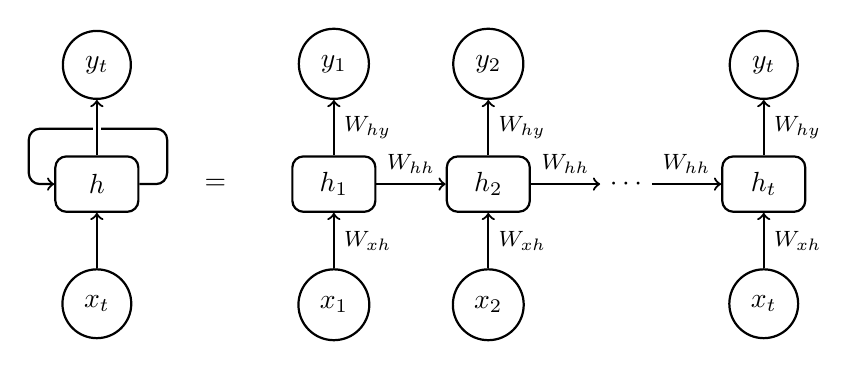
\begin{tikzpicture}[layer/.style={rectangle,draw, thick,align=center, minimum width=3em, minimum height=2em,inner sep=5pt,rounded corners=4},neuron/.style={circle,draw, thick,align=center,inner sep=5pt,rounded corners=4}, links/.style={->, thick}]
	
	\node[layer] (h-rolled) {$h$};
	\node[neuron, below = 2em of h-rolled] (input-rolled) {$x_t$};
	\node[neuron, above = 2em of h-rolled] (output-rolled) {$y_t$};
		\draw[links, rounded corners] (h-rolled.east) -| ++(1em,2em) -- ++(-5em,.0em) |- (h-rolled.west);
	\draw[links] (input-rolled) -- (h-rolled);
	\draw[line width=3pt,white] (h-rolled) -- (output-rolled);
	\draw[links] (h-rolled) -- (output-rolled);
	

	\node[right = 2em of h-rolled] (equals) {$=$};
	

	\node[layer, right = 2em of equals] (h-unrolled1) {$h_1$};
		\node[neuron, below = 2em of h-unrolled1] (input-unrolled1) {$x_1$};
	\node[neuron, above = 2em of h-unrolled1] (output-unrolled1) {$y_1$};
	\draw[links] (h-unrolled1) -- node[right] {\footnotesize $W_{hy}$} (output-unrolled1);
	\draw[links] (input-unrolled1) -- node[right] {\footnotesize $W_{xh}$} (h-unrolled1);
	
	
	
	\node[layer, right = 2.5em of h-unrolled1] (h-unrolled2) {$h_2$};
	\node[neuron, below = 2em of h-unrolled2] (input-unrolled2) {$x_2$};
	\node[neuron, above = 2em of h-unrolled2] (output-unrolled2) {$y_2$};
	
	\draw[links] (h-unrolled2) -- node[right] {\footnotesize $W_{hy}$} (output-unrolled2);
	\draw[links] (input-unrolled2) -- node[right] {\footnotesize $W_{xh}$} (h-unrolled2);
	
	\draw[links] (h-unrolled1) -- node[above] {\footnotesize $W_{hh}$} (h-unrolled2) ;
	
	\node[right = 2.5em of h-unrolled2] (dots) {$\cdots$}; 
	
	\draw[links] (h-unrolled2) -- node[above] {\footnotesize $W_{hh}$}(dots);
	
	\node[layer, right = 2.5em of dots] (h-unrolled3) {$h_t$};
	\node[neuron, below = 2em of h-unrolled3] (input-unrolled3) {$x_t$};
	\node[neuron, above = 2em of h-unrolled3] (output-unrolled3) {$y_t$};
	
	\draw[links] (h-unrolled3) -- node[right] {\footnotesize $W_{hy}$} (output-unrolled3);
	\draw[links] (input-unrolled3) -- node[right] {\footnotesize $W_{xh}$} (h-unrolled3);
	
	\draw[links] (dots) -- node[above] {\footnotesize $W_{hh}$}(h-unrolled3);
	
	\end{tikzpicture}

        \caption{Recurrent neural networks architecture}
        \label{fig:rnn}
    \end{figure}


 
\acrlong{cnn} (\acrshort{cnn}) have what is called convolutional layers. A convolutional layer takes an input (usually 2D images, but it can be 1D or 3D either) and apply a mathematical operation called convolution\footnote{Mathematically, the operation happening in a \acrshort{cnn} is called cross-corelation which is a bit different than the mathematical definition of a convolution. In Machine Learning literature those operations are called convolutions, this is the terminology that will be used here.}. Convolutions act like filters that extract features from raw data by recursively multiplying what is called kernel with the input data. Different kernels serve different purposes and can extract a wide variety of features from raw data. After feature extraction done by the convolutional layer, they serve as an input for a feedforward neural network (as described in section \ref{section:feedforward-neural-network}) for classification or regression.

\end{comment}